% !TEX root = ..\proposal.tex

\section{User Stories and Sprints}
    \label{sec:user_stories}

\subsection{Landing Page and Authentication/Registration}
    \label{subsec:landing_page}
    
The system workflow begins with a simple landing page whereby existing users are prompted to log-in and first-time users are prompted to sign-up with the system through entering a valid email address as well as choosing the preferred starting capital to trade with. The user stories in this epic are:\\

\noindent \textbf{User Story \#1:} As an unregistered user visiting the application’s landing page, I want to register using my email address and a password so that the system can remember me and my data.
\begin{itemize}
	\item \textit{\textbf{Definition of Done:} This story is considered done when the following information is inserted during registration: First name (mandatory), Last name (mandatory), Email (mandatory), Password (mandatory), Confirm password (mandatory).}
\end{itemize}

\noindent \textbf{User Story \#2:} As an unregistered user, I want to see an error message if something goes wrong when I attempt to register for an account so that I can recover from the error.
\begin{itemize}
	\item \textit{\textbf{Definition of Done:} This story is considered done when a visually distinguishable message is shown to the unregistered user, together with explanation what is incorrect (e.g. email missing an “@” symbol).} 
\end{itemize}

\noindent \textbf{User Story \#3:}  As an unregistered user, I want to receive a confirmation email once my registration is successful so that I can confirm that I successfully registered and able to log in with my chosen credentials.
\begin{itemize}
	\item \textit{\textbf{Definition of Done:} This story is considered done when an email is sent whenever a new user successfully registers to the application.} 
\end{itemize}

\noindent \textbf{User Story \#4:} As a registered user visiting the application’s landing page, I want to log in with my email address and password so that the system can authenticate me, and I can trust it. 
\begin{itemize}
	\item \textit{\textbf{Definition of Done:} This story is considered done when the following information is inserted during authentication: Email (mandatory) and Password (mandatory).} 
\end{itemize}

\noindent \textbf{User Story \#5:} As a registered user visiting the application’s landing page, I want to be able to reset my password if I’ve forgotten it so that I can retrieve my data.
\begin{itemize}
	\item \textit{\textbf{Definition of Done:} This story is considered done when the user can reset the password using the “Forgot Password” feature available on the landing page and can them login using the new set password.} 
\end{itemize}

\noindent \textbf{User Story \#6:} As a registered user, I want to see an error message if something goes wrong when I attempt to sign into my account so that I can recover from the error.
\begin{itemize}
	\item \textit{\textbf{Definition of Done:} This story is considered done when a visually distinguishable message is shown to the registered user, together with explanation what is incorrect (e.g. email missing an “@” symbol).} 
\end{itemize}

\noindent \textbf{User Story \#7:} As a user (registered and unregistered), I want to read the application’s terms of use and privacy policy so that I become familiar with what security features are implemented to protect my details.
\begin{itemize}
	\item \textit{\textbf{Definition of Done:} This story is considered done when links to the terms of user and privacy policy are added to the landing page and are accessible.} 
\end{itemize}

\noindent \textbf{User Story \#8:} As a user (registered and unregistered), I want to learn about the application and its features so that I get familiar with what features are available.
\begin{itemize}
	\item \textit{\textbf{Definition of Done:} This story is considered done when information about the application and its features are available to the user on the landing page.} 
\end{itemize}


\subsection{Search and Watchlist}
    \label{subsec:search_watchlist}

The watchlist is whereby the users can add or remove their preferred shares or those shares that are yet to prove to be profitable based on the trading strategy adopted. The watchlist offers sufficient information for the user to be able to act swiftly to prevent missing a valuable opportunity. The watchlist features buy and sell buttons for each stock to enhance the functionality of the overall system. To add new stocks to the watchlist, the user searches for the stock using the stock's symbol or company name from the search bar. The user stories in this epic are:\\

\noindent \textbf{User Story \#9:} As a user, I want to search for stocks by the stock’s symbol or company name so that I can see a list of stocks matching my search. 
\begin{itemize}
	\item \textit{\textbf{Definition of Done:} This story is considered done when a drop-down list appears whenever there is input into the search bar.} 
\end{itemize}

\noindent \textbf{User Story \#10:} s a user, I want to select a specific stock from the search results list so that I can view detailed information about the selected stock. 
\begin{itemize}
	\item \textit{\textbf{Definition of Done:} This story is considered done when individual items from the search results can be selected and information about the stock’s name, latest available price, day change and historical price chart.} 
\end{itemize}


\noindent \textbf{User Story \#11:} As a user, I want to add preferred stocks to my watchlist so that I can act swiftly and prevent missing valuable investment opportunities.
\begin{itemize}
	\item \textit{\textbf{Definition of Done:} This story is considered done when stocks can be added to the user’s watchlist page and detailed information about the stock’s name, latest available price, day change and historical price chart can be viewed for stocks in the watchlist.} 
\end{itemize}


\noindent \textbf{User Story \#12:} As a user, I want to remove stocks from my watchlist so that I can only focus on stocks which align with my investment strategy.
\begin{itemize}
	\item \textit{\textbf{Definition of Done:} This story is considered done when stocks can be removed from the user’s watchlist page along with all the detailed information about them.} 
\end{itemize}


\subsection{Market Orders}
    \label{subsec:market_orders}

Users can place market orders to simul-buy new stocks to expand their portfolio or simul-sell stocks they own. These orders are placed at a quoted price equivalent to the current price stock at the time the order is placed. The user stories in this epic are:\\

\noindent \textbf{User Story \#13:} As a user, I want to place a market order to buy a specific stock at the current market price so that I can add it to my portfolio of stocks.
\begin{itemize}
	\item \textit{\textbf{ Definition of Done:} This story is considered done when a buy button is added for stocks that quotes a specific price for buying.} 
\end{itemize}

\noindent \textbf{User Story \#14:} As a user placing an order to buy stocks, I want to specify the number of shares to be bought so that I won’t have to place different orders for the same stock.
\begin{itemize}
	\item \textit{\textbf{Definition of Done:} This story is considered done when an integer field is provided for the user to specify the number of shares to be purchased from a specific stock.} 
\end{itemize}

\noindent \textbf{User Story \#15:} As a user placing an order to buy stocks, I want to view the total value of the order I am placing so that I can have an insight on the amount I will spend.
\begin{itemize}
	\item \textit{\textbf{Definition of Done:} This story is considered done when the total order value is computed and displayed for the user in the market order page.} 
\end{itemize}

\noindent \textbf{User Story \#16:} As a user placing an order to buy stocks, I want to be able to proceed with the buy order so that the stocks can be added to my portfolio.
\begin{itemize}
	\item \textit{\textbf{Definition of Done:} This story is considered done when the proceed button is added to the buy order and clicking it updates the user’s portfolio with the purchased stocks.} 
\end{itemize}

\noindent \textbf{User Story \#17:} As a user placing an order to buy stocks, I want to be able to cancel the buy order so that I can have the flexibility to change by decision.
\begin{itemize}
	\item \textit{\textbf{Definition of Done:} This story is considered done when a cancel button is added to the buy order and clicking it cancels the order and returns the user to the portfolio dashboard.} 
\end{itemize}

\noindent \textbf{User Story \#18:} As a user placing an order to sell stocks, I want to be notified with an error message if the number of shares to be bought exceeds the available funds so that I can recover from such an error.
\begin{itemize}
	\item \textit{\textbf{Definition of Done:} This story is considered done when an error message is displayed when the value of order exceeds the available funds.} 
\end{itemize}

\noindent \textbf{User Story \#19:} As a user, I want to place a market order to sell a specific stock at the current market price so that I can remove it to my portfolio of stocks.
\begin{itemize}
	\item \textit{\textbf{Definition of Done:} This story is considered done when a sell button is added for stocks that quotes a specific price for selling.} 
\end{itemize}

\noindent \textbf{User Story \#20:} As a user placing an order to sell stocks, I want to specify the number of shares to be sold so that I won’t have to place different orders for the same stock.
\begin{itemize}
	\item \textit{\textbf{Definition of Done:} This story is considered done when an integer field is provided for the user to specify the number of shares to be sold from a specific stock.} 
\end{itemize}

\noindent \textbf{User Story \#21:} As a user placing an order to sell stocks, I want to view the total value of the order I am placing so that I can have an insight on the amount I will receive.
\begin{itemize}
	\item \textit{\textbf{Definition of Done:} This story is considered done when the total order value is computed and displayed for the user in the market order page.} 
\end{itemize}

\noindent \textbf{User Story \#22:} As a user placing an order to sell stocks, I want to be able to proceed with the sell order so that the stocks can be removed from my portfolio.
\begin{itemize}
	\item \textit{\textbf{Definition of Done:} This story is considered done when the proceed button is added to the sell order and clicking it updates the user’s portfolio and removes the sold stocks.} 
\end{itemize}

\noindent \textbf{User Story \#23:} As a user placing an order to sell stocks, I want to be able to cancel the sell order so that I can have the flexibility to change by decision.
\begin{itemize}
	\item \textit{\textbf{Definition of Done:} This story is considered done when a cancel button is added to the s order and clicking it cancels the order and returns the user to the portfolio dashboard.} 
\end{itemize}

\noindent \textbf{User Story \#24:} As a user placing an order to sell stocks, I want to be notified with an error message if the number of shares to be sold exceeds the owned shares so that I can recover from such an error.
\begin{itemize}
	\item \textit{\textbf{Definition of Done:} This story is considered done when an error message is displayed when the number of shares specified exceeds the shares owned.} 
\end{itemize}

\subsection{Portfolio Dashboard}
    \label{subsec:portfolio_dashboard}

The portfolio dashboard comprises the most intriguing yet critical page for the user. The portfolio dashboard allows the user to observe each holding separately in terms of the stock name, number of shares held, the average price of entry for the aggregated positions, the current share price, and the nominal  gain. Additionally, the total gain is depicted within a graph that shows the day closing portfolio value to observe the portfolio growth over time. Finally, from the portfolio dashboard, the user has the convenience of buying more positions and closing open positions (or part of open positions) to increase the platform versatility. The user stories in this epic are:\\

\noindent \textbf{User Story \#25:} As a user, I want to view aggregate statistics about my portfolio including the current portfolio value, the day return from the portfolio as well as the total return so that I can have an overview about the current portfolio state.
\begin{itemize}
	\item \textit{\textbf{Definition of Done:} This story is considered done when the portfolio dashboard includes information on the current portfolio value, the day return from the portfolio as well as the total return.} 
\end{itemize}
\noindent \textbf{User Story \#26:} As a user, I want to view a chart displaying the historical performance of my portfolio so that I would gain insight on whether my investment strategies have been working well or not.
\begin{itemize}
	\item \textit{\textbf{Definition of Done:} This story is considered done when the portfolio dashboard includes a chart showing the portfolio’s historical performance.} 
\end{itemize}
\noindent \textbf{User Story \#27:} As a user, I want to view the constituents of my portfolio including the symbol and company name of the stocks I own as well as details on the number of shares, the total cost, current value and return for each stock.
\begin{itemize}
	\item \textit{\textbf{Definition of Done:} This story is considered done when the portfolio dashboard includes details about the portfolio constituents including the symbol and company name of the stocks I own as well as details on the number of shares, the total cost, current value and return for each stock.} 
\end{itemize}
\noindent \textbf{User Story \#28:} As a user viewing the portfolio dashboard, I want to buy more shares of a specific stock I already own so that I can expand my portfolio.
\begin{itemize}
	\item \textit{\textbf{Definition of Done:} This story is considered done when a buy button is displayed next to each constituent of the portfolio allowing the user to place a market order to buy more from the stock.} 
\end{itemize}
\noindent \textbf{User Story \#29:} As a user viewing the portfolio dashboard, I want to sell shares of a specific stock I already own so that I can get rid of stocks that do not align with my investment strategy any longer.
\begin{itemize}
	\item \textit{\textbf{Definition of Done:} This story is considered done when a sell button is displayed next to each constituent of the portfolio allowing the user to place a market order to sell from the stock.} 
\end{itemize}

\subsection{Account Settings}
    \label{subsec:account_settings}

On the account settings side, the user can change the password or details and log-out from the system. The user stories in this epic are:\\

\noindent \textbf{User Story \#30:} As a user, I can change my first name, last name and password because my preferences might have changed since creating the account.
\begin{itemize}
	\item \textit{\textbf{Definition of Done:} This story is considered done when the user can change the first name, last name, and password and the updated data are reflected when the user logs in.} 
\end{itemize}

\noindent \textbf{User Story \#31:} As a user, I can sign out from the application when I am done using it so that I keep my data secure.
\begin{itemize}
	\item \textit{\textbf{Definition of Done:} This story is considered done when the user can log out from the application and all authentication information is removed.} 
\end{itemize}

\subsection{Sprints Schedule and First Sprint}
    \label{subsec:sprint_schedule}

{\color{red} DEFINE THE START AND END DATES FOR ALL SPRINTS ENVISAGED DURING TERM. ENSURE THAT THE SPRINTS ALLOW YOU TO UNDERTAKE A DEMO IN EACH OF WEEK 5 AND WEEK 8 AS WELL AS A RETROSPECTIVE BEFORE EACH OF THE LABS IN WEEKS 7 AND 9.\\
	
\noindent IDENTIFY USER STORIES IN SCOPE FOR THE FIRST SPRINT WITH SCREENSHOTS SHOWING ALL USER STORIES ALLOCATED TO THE FIRST SPRINT IN JIRA.}

\newpage

\begin{landscape}
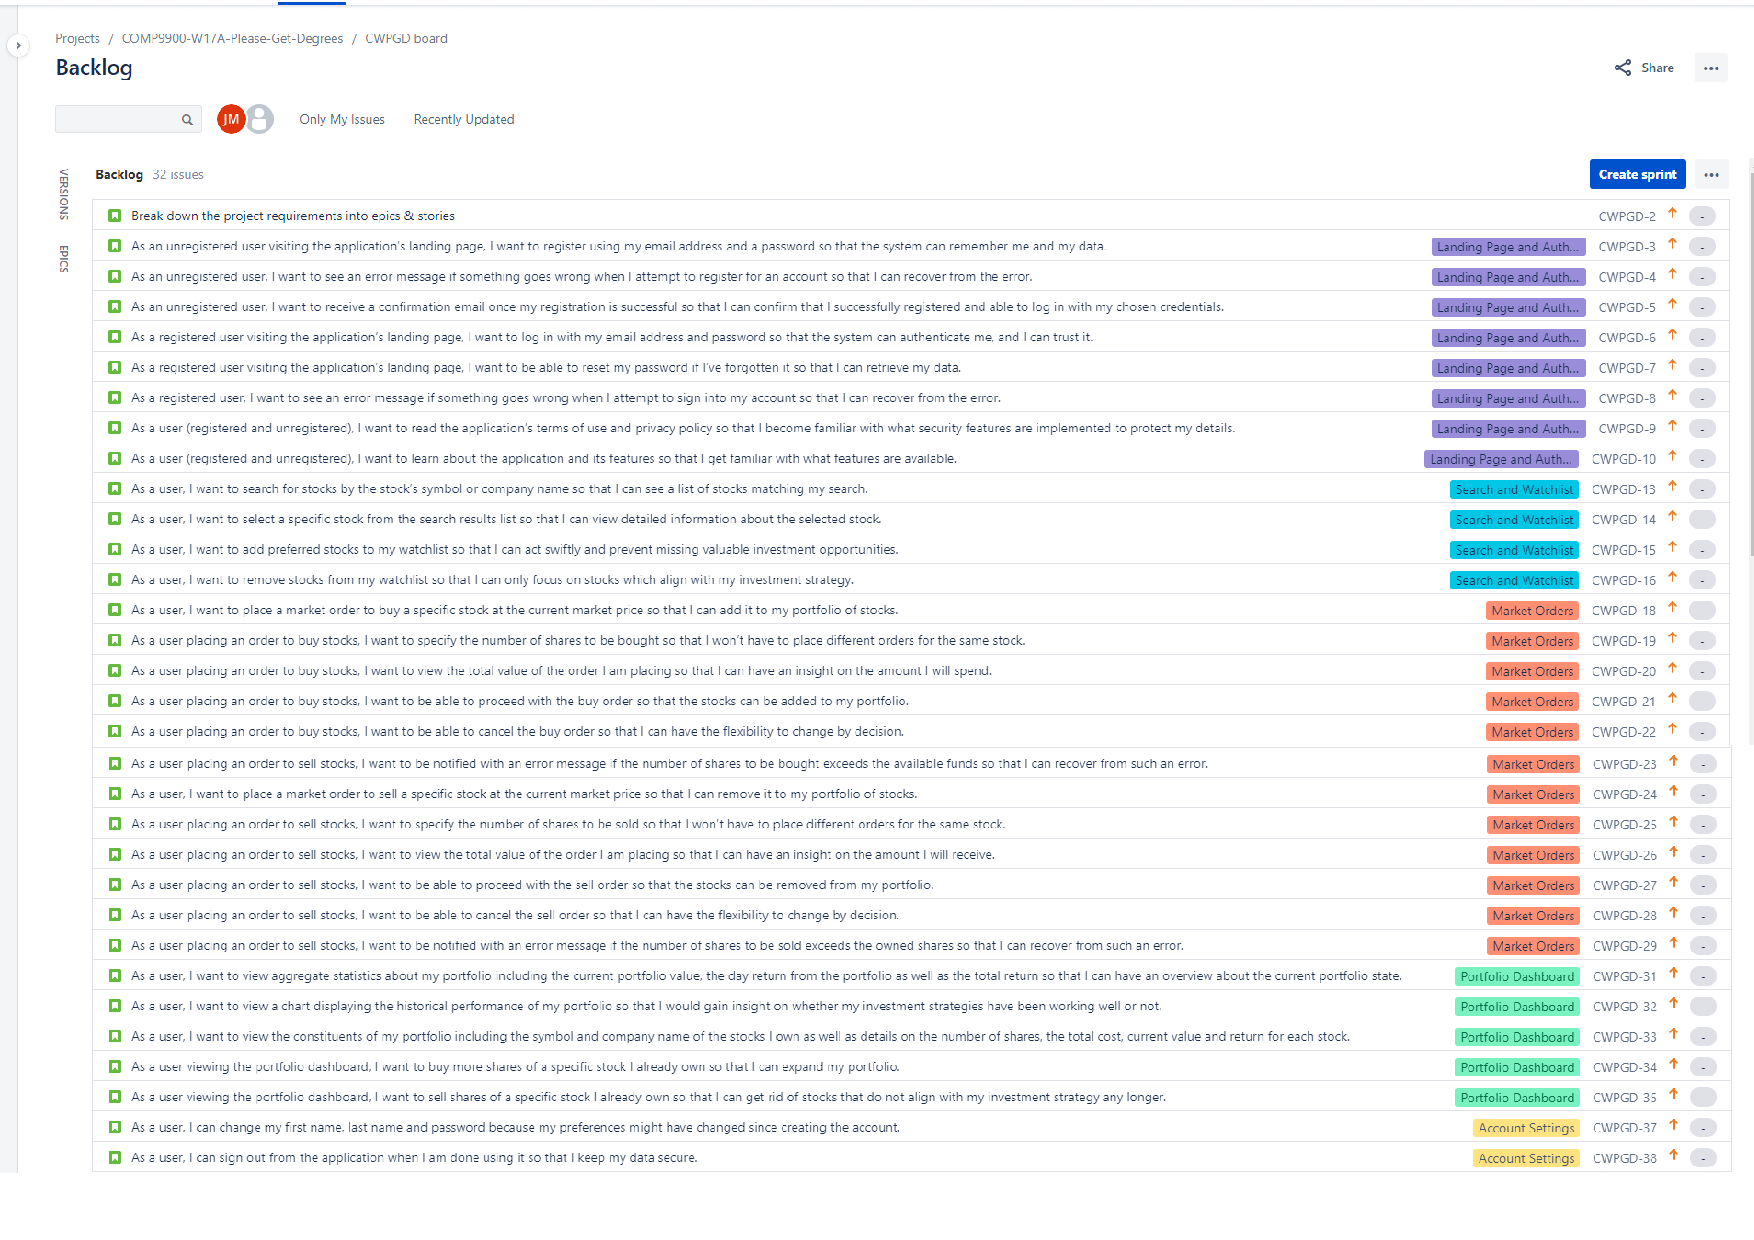
\includepdf[landscape=true]{./3_user_stories/Jira_Screenshot.pdf}
\end{landscape}

\newpage